
%\begin{figure}[htb]
%    \centering
%    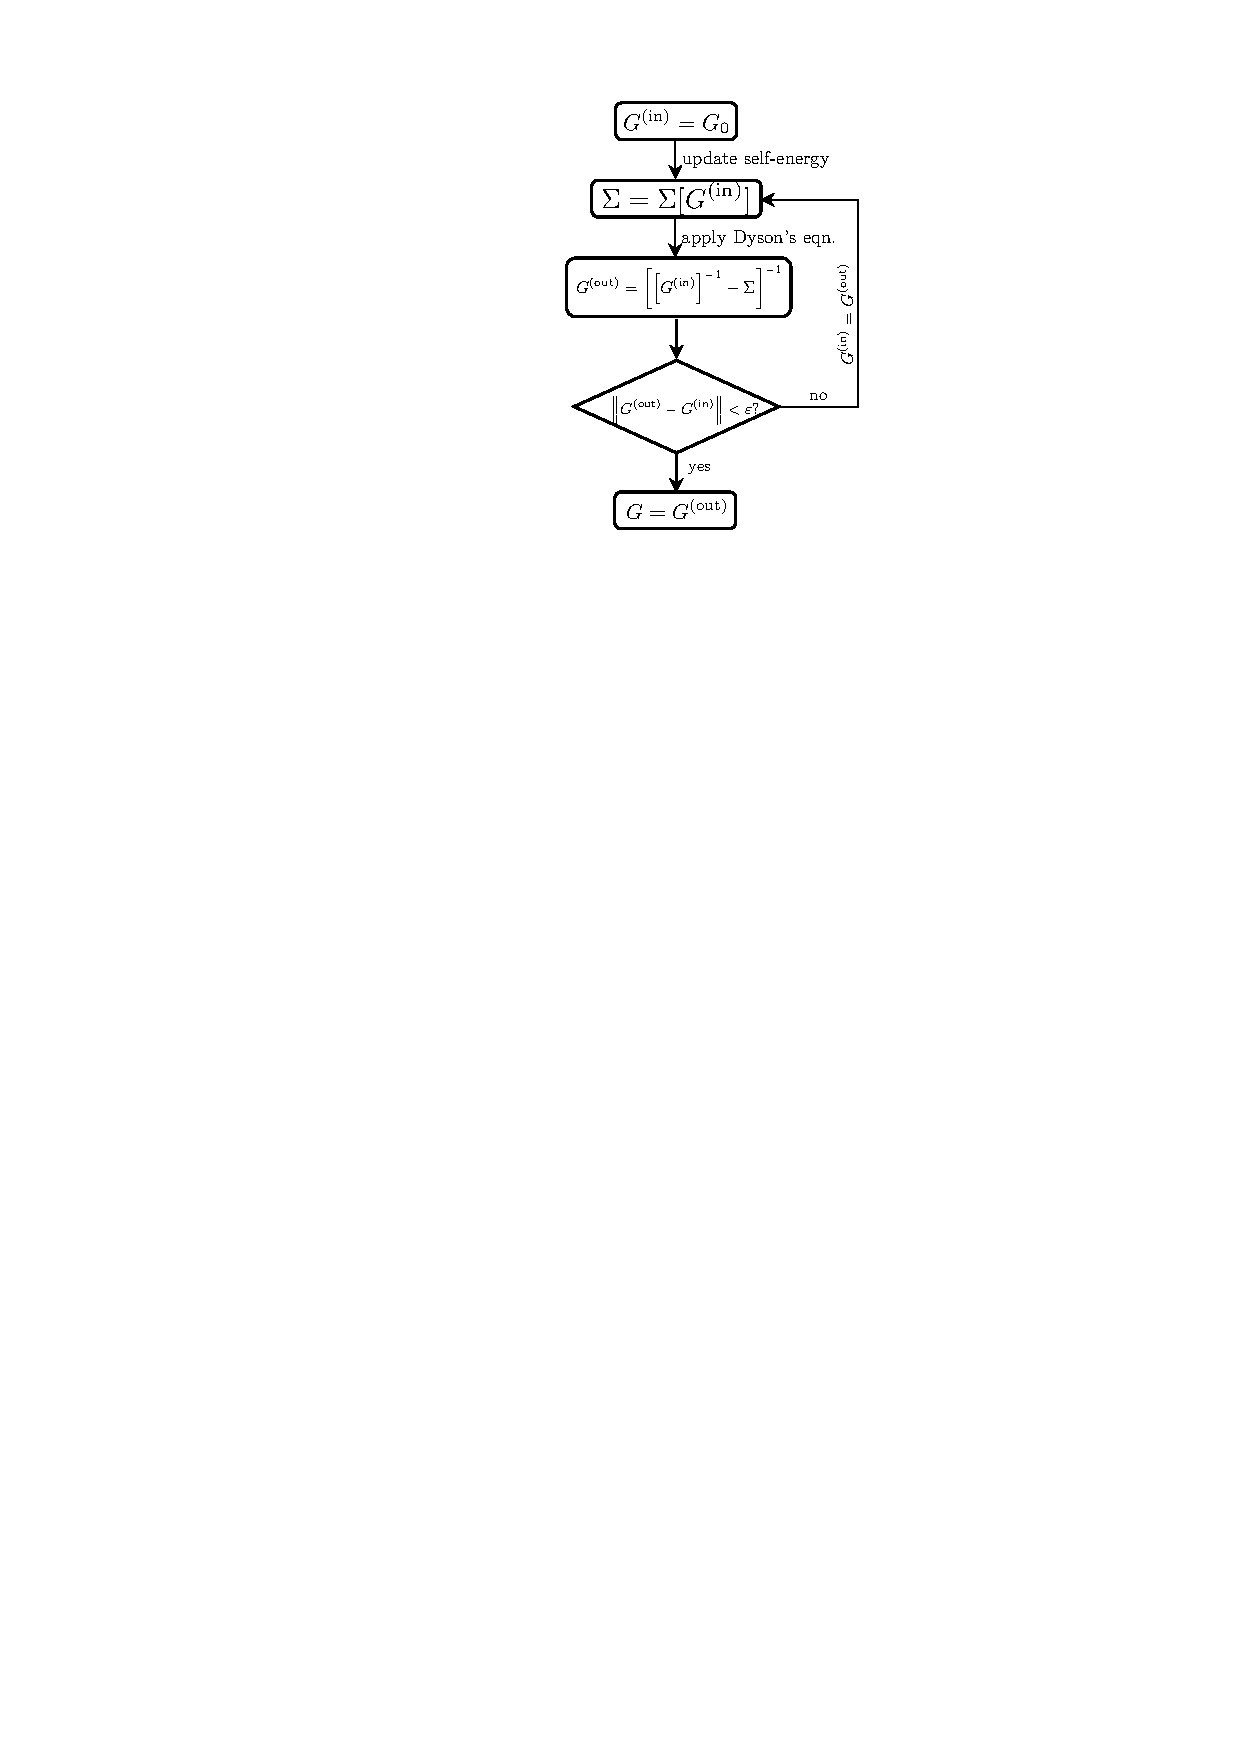
\includegraphics[width=0.3\textwidth]{dyson.pdf}
%    \caption{Flowchart illustrating the self-consistent procedure for solving the Dyson's equation in many-body physics.}
%    \label{fig:dyson}
%    \end{figure}


The many-body perturbation theory, which utilises the mathematical tool of Green's function\cite{economou2006green} provides the systematic framework to treat the electron-correlation effects in complex material systems. Here, we will provide a gentle introduction on many-body Green's function. 


\begin{wrapfigure}[27]{r}{0.3\textwidth}
  \begin{center}
    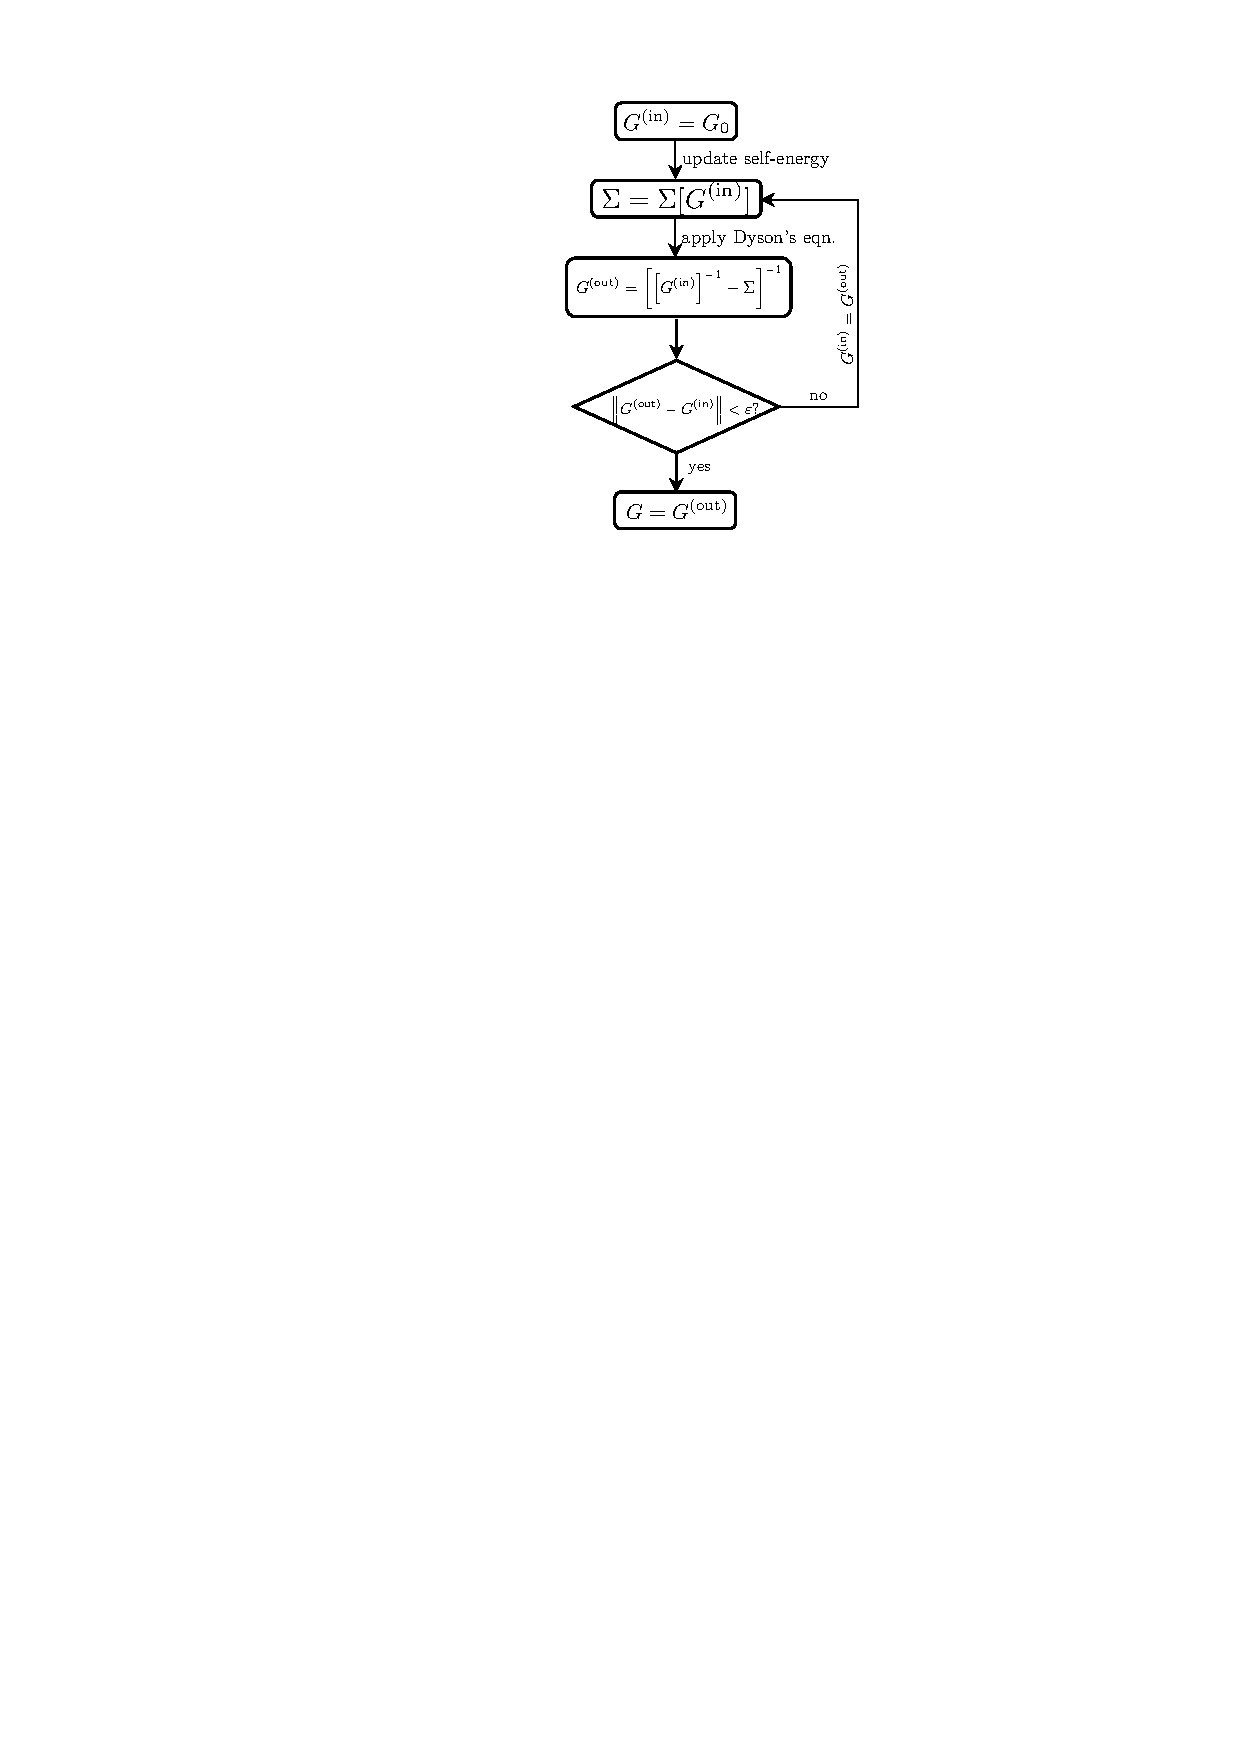
\includegraphics[width=0.3\textwidth]{dyson.pdf}
    \caption{Flowchart illustrating the self-consistent procedure for solving the Dyson's equation in many-body physics.}
    \label{fig:dyson_solution}
  \end{center}
\end{wrapfigure}

In the time-dependent formalism, the Green's function $G(\bm{r},\bm{r}^\prime, t,t^\prime)$ is a function that describes the evolution of the amplitude of electron wavefunction from $(\bm{r}^\prime,t^\prime)$ to $(\bm{r},t)$ in the time-position space under the influence of the Coulomb interactions from all the other electrons. Here, we are interested in its Fourier transformation into the energy domain $G(\bm{r},\bm{r}^\prime,\omega)$, which is usually defined in the complex plane of energy. This can be seen from the Lehman representation of the Green's function,\cite{economou2006green}  for example, giving the quantum states of the system described by a set of basis functions $\{\phi_i(\bm{r})\}$ with $\{\varepsilon_i\}$ being the corresponding eigenenergies, we have,
\begin{equation}
    \label{eq:Lehman}
    G(\bm{r},\bm{r}^\prime,\omega)=\sum_{i}\langle\phi_i|\phi_i\rangle \left[\frac{\Theta(\varepsilon_i-E_F )}{\hbar\omega-(\varepsilon_i -i\eta)}+\frac{\Theta(E_F-\varepsilon_i )}{\hbar\omega-(\varepsilon_i +i\eta)}\right],
\end{equation}
in which $E_F$ is the Fermi energy,  $\Theta$ is the Heaviside step function and $\eta\to0^{+}$. The poles of the Green's function, which occur at $\{\varepsilon_i\}$, correspond to the quasiparticle energies, can be directly matched with the  experimentally measured EA and IP. 



Apparently, the quasiparticle energies $\{\varepsilon_i\}$ are supposed to be obtained from solving the full many-body Schr\"{o}dinger equation, from which the corresponding Green's function can be defined according to \cref{eq:Lehman}, but we know this is generally not possible to achieve. This problem is solved by applying the \emph{Dyson's equation}.\cite{dyson1949} Starting from the non-interacting single-particle Green's function $G_0(\omega)$, which can be constructed using the Lehman's representation [\cref{eq:Lehman}] with, for example, the Kohn-Sham orbitals and energies, the corresponding many-body Green's function $G(\omega)$ can be determined with the knowledge of the self-energy $\Sigma(\omega)$ as:
\begin{equation}
    \label{eq:Dyson_equation}
    G(\omega)=G_0(\omega)+G_0(\omega)\Sigma(\omega)G(\omega).
\end{equation}


The Dyson's equation is usually solved iteratively until self-consistency is reached, for which \cref{fig:dyson_solution} illustrates the general procedure behind. It can be seen that the self-energy $\Sigma(\omega)$ itself is also a function of the Green's function. More specifically, as discussed later,  the self-energy $\Sigma(\omega)$ is the product of the Green's function $G(\omega)$ and the screened Coulomb interaction $W(\omega)$, thus taking into account the mutual interaction between an electron and its surrounding polarisation cloud, leading to the name of $GW$ approach. 

